\documentclass[conference]{IEEEtran}
\usepackage{times}
\usepackage{amsmath,amssymb}
\usepackage{graphicx}
\usepackage{booktabs}
\usepackage{multirow}
\usepackage[numbers,sort&compress]{natbib}
\usepackage{url}
\usepackage[bookmarks=true,hidelinks]{hyperref}

\hypersetup{
  pdftitle={Differentiable 3-Axis CNC Machining: Co-Optimizing Toolpaths and Feedrates via Smooth-to-Hard Surrogate Gradients and Residual Reinforcement Learning},
  pdfauthor={Anonymous Authors},
  pdfsubject={Robotics; Computer-Aided Manufacturing; Differentiable Simulation; Reinforcement Learning},
  pdfkeywords={CNC Machining, Differentiable Simulation, Trajectory Optimization, Reinforcement Learning, Toolpath Planning}
}

\begin{document}

\title{Differentiable 3-Axis CNC Machining: Co-Optimizing Toolpaths and Feedrates via Smooth-to-Hard Surrogate Gradients and Residual Reinforcement Learning}

\author{Author Names Omitted for Anonymous Review}

\maketitle

\begin{abstract}
Generating physically optimal toolpaths for 3-axis Computer Numerical Control (CNC) milling requires reasoning over long-horizon trajectories in which every cutting pass permanently mutates the in-process workpiece (IPW) geometry and governs subsequent cutter-workpiece engagement (CWE) loads. Classical computer-aided manufacturing (CAM) relies on conservative geometric offset heuristics and constant feedrates because Boolean solid-modeling kernels are discontinuous—yielding zero gradients during air-cutting and undefined derivatives at stock boundaries—while naive geometry-only optimization under exact-stop kinematics fails to exploit real CNC corner blending or respect volumetric chip-load limits. We present \textbf{DiffCAM}, an MIT-licensed, GPU-accelerated dual-mode differentiable 3-axis milling framework that couples exact Boolean swept-cylinder signed distance field (SDF) carving with a log-sum-exp smooth relaxation, Straight-Through Estimator (STE) stiffness continuation, acceleration-bounded junction corner blending aligned with NIST RS274 (\texttt{G64 P0.05}) and Haas Next-Gen Control (\texttt{G187 P2 E0.05}), and an analytical Peak Material Removal Rate (MRR) barrier. Seeded by modular clean-room CAM engines spanning Facing, Pocket, trochoidal Adaptive, and Contour operations ($37$--$370$ segments) and parameterized via a drift-free, wall-clearance-weighted \texttt{JointPathFeedSpline}, we conduct a controlled study comparing first-order differentiable trajectory and policy optimization (\texttt{STE-Continuation-Adam}, \texttt{Annealed-Adam}, \texttt{DiffPolicy-SHAC}) against zero-order reinforcement learning and black-box search (\texttt{Hard-PPO}, \texttt{Hard-CEM}, \texttt{Hard-CMA-ES}) across 16 tasks under a strict 64-call simulator budget. Smooth-to-hard continuation (\texttt{STE-Continuation-Adam} and \texttt{Annealed-Adam}) reduces mean cycle time by $\mathbf{42.0 \pm 13.5\%}$ and $\mathbf{43.0 \pm 15.7\%}$ ($122.2\text{ s} \to 73.9\text{ s}$) at $\mathbf{100\%}$ hard feasibility—nearly $4\times$ the gain of evolutionary search ($9.3\%$--$11.3\%$)—while first-order \texttt{DiffPolicy-SHAC} achieves $2.0\times$ the speedup of zero-order \texttt{Hard-PPO} ($\mathbf{37.0\%}$ vs.\ $\mathbf{18.5\%}$) and leads all methods on enclosed \texttt{Pocket} roughing ($\mathbf{32.1\%}$). Ablations show that removing our volumetric MRR barrier triggers $+136.7\%$ cutter overload, and independent verification across 6 industrial CNC dialects ($48/48$ pass), a $0.125\text{ mm}$ posted G-code evaluator, and containerized \texttt{CAMotics v1.2.0} certifies $8/8$ watertight STL solids with $0.00\text{ mm}^3$ gouge, $0.00\text{ mm}^3$ uncut residual, and interactive 3D stock-and-toolpath simulation bundles.
\end{abstract}

\IEEEpeerreviewmaketitle

\section{Introduction}
\label{sec:intro}

Subtractive CNC machining remains the backbone of precision mechanical manufacturing, yet toolpath generation is still dominated by purely geometric rules devised decades ago~\cite{held1991pocket,altintas2012manufacturing}. Unlike collision-free robot motion planning in static environments, 3-axis milling is a history-dependent, irreversible manipulation process over a continuous volumetric field: every millimeter traveled by the rotating endmill permanently carves the in-process workpiece (IPW), determining the radial and axial cutter-workpiece engagement (CWE) encountered by future passes~\cite{rauch2009trochoidal,suh2008cnc}. Consequently, standard industrial CAM packages decouple toolpath topology (e.g., zig-zag facing, offset pocketing, trochoidal clearing, exterior contouring) from conservative, worst-case constant feedrates chosen to survive full-width slotting corners—leaving substantial machine productivity unrealized during partial-engagement cuts and air-repositioning transitions.

\begin{figure*}[t]
  \centering
  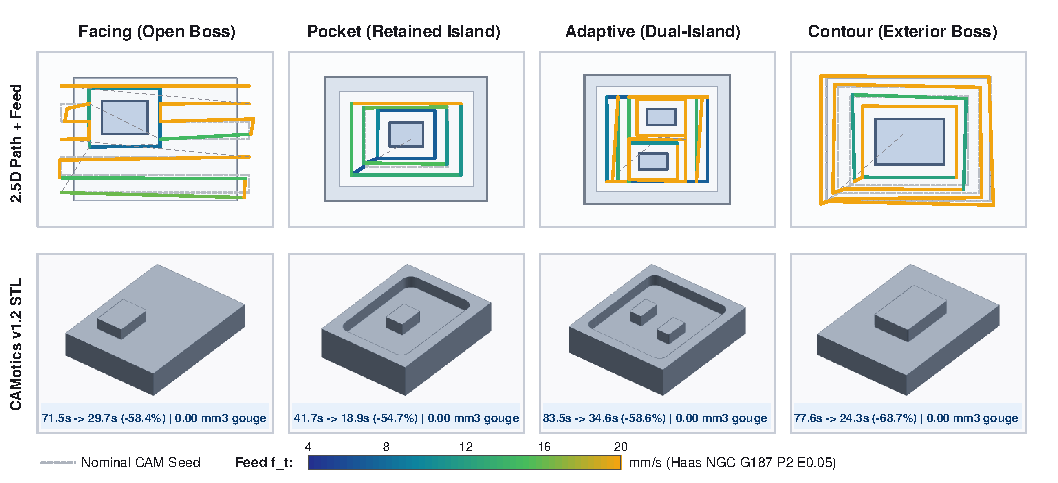
\includegraphics[width=\textwidth]{figures/fig1_hero_camotics.pdf}
  \vspace{-1.6em}
  \caption{\textbf{DiffCAM joint 2.5D toolpath and feedrate co-optimization certified in CAMotics v1.2.0.} \emph{Top row:} Representative held-out test parts across four modular MIT clean-room CAM strategy families showing stock billets, retained islands/bosses, dashed gray nominal CAM seeds ($37$--$370$ segments), and optimized \texttt{STE-Continuation-Adam} trajectories colored by per-segment feedrate $f_t \in [2.8, 20.0]\text{ mm/s}$ under Haas Next-Gen Control corner blending (\texttt{G54}, \texttt{G187 P2 E0.05}). \emph{Bottom row:} 4$\times$-MSAA isometric renderings of the closed, watertight binary STL meshes reconstructed directly by containerized \texttt{CAMotics v1.2.0} ($0.25\text{ mm}$ grid) from posted Haas NGC G-code, achieving $29.4\%$--$60.9\%$ cycle-time reductions on these four parts ($39.5\%$ mean across all 8 test parts) with $0.00\text{ mm}^3$ target gouge, $0.00\text{ mm}^3$ residual, and exact STL volume identity with nominal CAM.}
  \label{fig:hero}
  \vspace{-0.8em}
\end{figure*}

Bridging modern gradient-based trajectory optimization and reinforcement learning (RL) with CNC milling faces three coupled obstacles:
\begin{enumerate}
  \item \textbf{Discontinuous Boolean Material Removal:} In solid modeling and dexel/voxel kernels~\cite{vanhook1986dexel,coffland2021camotics}, subtracting a swept tool volume $\psi_{\text{tool}}$ from stock SDF $\phi_t$ via $\phi_{t+1}(\mathbf{x}) = \max(\phi_t(\mathbf{x}), -\psi_{\text{tool}}(\mathbf{x}))$ yields identically zero spatial gradients when a segment cuts air and non-differentiable kinks at cutter engagement boundaries~\cite{shapiro2007rfunctions}.
  \item \textbf{Surrogate Bias and Cumulative Drift:} Naive smooth relaxations of $\max(\cdot,\cdot)$ introduce volumetric occupancy inflation at low stiffness $k$, causing optimizers to hallucinate phantom material removal that fails exact Boolean evaluation~\cite{suh2022differentiable,metz2021gradients}. Simultaneously, parameterizing multi-pass toolpaths via relative segment deltas $\Delta \mathbf{p}_t$ induces $O(T)$ cumulative position variance across $T \sim 37\text{--}370$ segments, slamming interior passes into blueprint walls.
  \item \textbf{Controller-Blind Kinematics:} Optimizing path length under constant feedrates and exact-stop (\texttt{G61}) assumptions stalls when part tolerances fix the required pass count, whereas naively maximizing feedrates without volumetric engagement feedback causes catastrophic cutter overload ($\text{MRR}_t \gg \text{MRR}_{\max}$) or mismatches physical CNC corner-rounding deceleration~\cite{erkorkmaz2001highspeed,kramer2000rs274ngc}.
\end{enumerate}

These challenges motivate a central question in differentiable physical AI: \emph{when initialized from valid topological CAM seeds under a tight simulation budget, how do first-order analytical gradients through a smoothed-to-hard cutting simulator compare against zero-order RL and evolutionary strategies operating directly on exact Boolean cutting?}

To answer this question rigorously, we introduce \textbf{DiffCAM} (Fig.~\ref{fig:hero}), an end-to-end differentiable 3-axis milling simulator, trajectory optimizer, and residual RL benchmark built in Taichi~\cite{hu2020difftaichi}. Our primary contributions are fourfold:
\begin{itemize}
  \item \textbf{Dual-Mode Swept-CSG Simulation with STE Continuation:} We formulate a GPU-accelerated 3D SDF simulator supporting both exact Boolean material removal and a log-sum-exp smooth surrogate, paired with a Straight-Through Estimator (STE)~\cite{bengio2013estimating} stiffness schedule ($k: 25 \to 90$) and exact hard-feasibility checkpointing that eliminates soft-to-hard occupancy drift.
  \item \textbf{Blended CNC Kinematics and Volumetric MRR Barrier:} We co-optimize continuous 2.5D XY toolpaths and per-segment feedrates under a differentiable acceleration-bounded junction blending model aligned with \texttt{RS274} \texttt{G64 P0.05} and Haas Next-Gen Control \texttt{G187 P2 E0.05}, constrained by differentiable pre-cut chip-volume Peak MRR, analytical wall-gouge, holder-collision, and rapid-clearance barriers.
  \item \textbf{Clean-Room CAM Engines, Drift-Free Co-Parameterization, and Controlled RL Study:} We build modular MIT clean-room CAM engines (\texttt{facing}, \texttt{pocket}, trochoidal \texttt{adaptive}, \texttt{contour}), introduce an analytical wall-clearance-weighted \texttt{JointPathFeedSpline} that eliminates $O(T)$ cumulative delta drift while pinning plunge/retract and finishing boundaries, and compare first-order \texttt{STE-Continuation-Adam}, \texttt{Annealed-Adam}, and \texttt{DiffPolicy-SHAC}~\cite{xu2022accelerated} against zero-order \texttt{Hard-PPO}~\cite{schulman2017proximal}, \texttt{Hard-CEM}~\cite{rubinstein2004cem}, and \texttt{Hard-CMA-ES}~\cite{hansen2001cmaes} under strict simulator-call parity.
  \item \textbf{Multi-Controller G-Code, CAMotics STL, and Interactive 3D Simulation:} Every held-out test solution is post-processed across 6 industrial CNC dialects (\texttt{RS274}, Haas NGC \texttt{O01001}--\texttt{O01008}, \texttt{FANUC}, \texttt{Robodrill}, \texttt{Makino}, \texttt{Mazak}), exported to native \texttt{.rustcnc}, \texttt{.camotics}, and WebGL 3D stock-and-toolpath simulators, and certified by both a $0.125\text{ mm}$-step evaluator and containerized \texttt{CAMotics v1.2.0}~\cite{coffland2021camotics} ($48/48$ dialect pass, $8/8$ watertight STLs, $0.00\text{ mm}^3$ gouge, $0.00\text{ mm}^3$ residual, and $36.2\%$ aggregate / $39.5\%$ mean test cycle-time reduction).
\end{itemize}

\section{Related Work}
\label{sec:related}

\textbf{Geometric CAM and Engagement-Aware Toolpaths.}
Classical pocket and contour milling rely on 2D Voronoi medial-axis offsets~\cite{held1991pocket} and direction-parallel rastering, which suffer from sharp radial engagement spikes in concave corners. Trochoidal and adaptive clearing strategies~\cite{rauch2009trochoidal,altintas2012manufacturing} bound radial immersion via circular or cycloidal loops, while solid verification engines use Z-buffer dexels~\cite{vanhook1986dexel}, R-functions~\cite{shapiro2007rfunctions}, or octree marching-cubes isosurfaces as in \texttt{CAMotics}~\cite{coffland2021camotics}. However, these forward geometric kernels are non-differentiable, preventing direct gradient-based co-adaptation of waypoint geometry and feed schedules to part-specific stock state.

\textbf{CNC Corner Blending and Feedrate Scheduling.}
Physical CNC interpolators avoid coming to a complete stop at every linear \texttt{G1} block junction (\texttt{G61}) by blending adjacent velocity vectors within a user-specified path-deviation tolerance—standardized as \texttt{G64 P}$e$ in NIST \texttt{RS274NGC}~\cite{kramer2000rs274ngc} and \texttt{G187 P2 E}$e$ on Haas Next-Gen Control~\cite{suh2008cnc,erkorkmaz2001highspeed}. Classical feedrate scheduling optimizes speed along a \emph{frozen} reference path under axis acceleration or cutting-force bounds~\cite{altintas2012manufacturing,erkorkmaz2001highspeed}. Conversely, optimizing path geometry under frozen feeds yields negligible speedup when feature walls lock pass topology. DiffCAM unifies both regimes by backpropagating simultaneously through blended junction kinematics, swept chip-volume engagement, and waypoint positions.

\textbf{Differentiable Physics vs.\ Zero-Order RL.}
Differentiable simulators such as \texttt{DiffTaichi}~\cite{hu2020difftaichi} and \texttt{Brax}~\cite{freeman2021brax} enable low-variance first-order trajectory optimization and short-horizon analytic actor-critic training (\texttt{SHAC})~\cite{xu2022accelerated}. Yet Suh et al.~\cite{suh2022differentiable} and Metz et al.~\cite{metz2021gradients} showed that stiff contact discontinuities can induce high gradient variance or surrogate bias, allowing randomized zero-order estimators such as \texttt{PPO}~\cite{schulman2017proximal,schulman2016gae}, \texttt{CEM}~\cite{rubinstein2004cem}, and \texttt{CMA-ES}~\cite{hansen2001cmaes} to remain competitive. By combining log-sum-exp CSG smoothing with Straight-Through Estimator (STE) evaluation~\cite{bengio2013estimating} and stiffness continuation, DiffCAM preserves high gradient signal-to-noise ratio ($\text{SNR} \in [30.5, 62.2]$) across $37$--$370$ cutting segments while guaranteeing zero surrogate gap at deployment.

\section{Differentiable 3-Axis Milling Formulation}
\label{sec:formulation}

\subsection{Dual-Mode Swept-Cylinder SDF Material Removal}
We represent the 3D stock billet on a uniform Eulerian grid $\Omega \subset \mathbb{R}^3$ of voxel pitch $\Delta x$ with signed distance values $\phi_t : \Omega \to \mathbb{R}$ after segment $t \in \{0,\dots,T\}$, following the convention $\phi_t(\mathbf{x}) < 0$ inside solid material and $\phi_t(\mathbf{x}) > 0$ in empty space. Given a flat-end cylindrical cutter of radius $R$, flute length $L_{\text{flute}}$, holder clearance height $L_{\text{clear}}$, and holder shank radius $R_{\text{holder}} > R$ moving linearly from $\mathbf{p}_{t-1} \in \mathbb{R}^3$ to $\mathbf{p}_t \in \mathbb{R}^3$, let $\tau^\star(\mathbf{x}) = \operatorname{clip}\!\big(\frac{(\mathbf{x} - \mathbf{p}_{t-1})\cdot \Delta\mathbf{p}_t}{\|\Delta\mathbf{p}_t\|_2^2 + \varepsilon}, 0, 1\big)$ denote the closest-point parameter along $\Delta\mathbf{p}_t = \mathbf{p}_t - \mathbf{p}_{t-1}$, with interpolated tool-tip reference $\mathbf{c}_t(\mathbf{x}) = \mathbf{p}_{t-1} + \tau^\star(\mathbf{x})\Delta\mathbf{p}_t$. The local swept cutting-flute SDF is
\begin{equation}
  \begin{aligned}
    \psi_{\text{tool}}(\mathbf{x}; \mathbf{p}_{t-1}, \mathbf{p}_t) =\;& \max\Big(
      \|\mathbf{x}^{xy} - \mathbf{c}_t^{xy}(\mathbf{x})\|_2 - R, \\
      &c_t^z(\mathbf{x}) - x^z,\; x^z - \big(c_t^z(\mathbf{x}) + L_{\text{flute}}\big)\Big).
  \end{aligned}
  \label{eq:swept_tool}
\end{equation}

In \textbf{exact hard Boolean mode}, material subtraction updates the IPW via the exact CSG difference:
\begin{equation}
  \phi_t^{\text{hard}}(\mathbf{x}) = \max\!\big(\phi_{t-1}^{\text{hard}}(\mathbf{x}),\; -\psi_{\text{tool}}(\mathbf{x}; \mathbf{p}_{t-1}, \mathbf{p}_t)\big).
  \label{eq:hard_csg}
\end{equation}
Because $\max(a,b)$ has zero derivative with respect to inactive arguments and a discontinuous subgradient along $a = b$, we pair Eq.~\eqref{eq:hard_csg} with a numerically stabilized \textbf{smooth log-sum-exp relaxation} controlled by inverse-temperature stiffness $k > 0$:
\begin{equation}
  \begin{aligned}
    \phi_t^{(k)}(\mathbf{x}) &= \max_k\!\big(\phi_{t-1}^{(k)}(\mathbf{x}), -\psi_{\text{tool}}(\mathbf{x})\big) \\
    &= m + \frac{1}{k}\log\!\Big(e^{k(\phi_{t-1}^{(k)}(\mathbf{x}) - m)} + e^{k(-\psi_{\text{tool}}(\mathbf{x}) - m)}\Big),
  \end{aligned}
  \label{eq:soft_csg}
\end{equation}
where $m = \max(\phi_{t-1}^{(k)}(\mathbf{x}), -\psi_{\text{tool}}(\mathbf{x}))$. Smooth voxel occupancy is mapped via the logistic sigmoid $\sigma_k(\phi) = (1 + e^{k\phi})^{-1} \in (0,1)$, which converges pointwise to the hard indicator $\mathbb{I}[\phi < 0]$ as $k \to \infty$ while providing dense, analytically differentiable reverse-mode sensitivities $\partial \mathcal{L}_k / \partial \mathbf{p}_t$ across the $\mathcal{O}(1/k)$ boundary layer.

\subsection{Straight-Through Estimator and Stiffness Continuation}
Optimizing $\mathcal{L}_k$ at a fixed low stiffness (e.g., $k \le 20$) suffers from severe \emph{surrogate occupancy drift}: the $\frac{\log 2}{k}$ additive shift in Eq.~\eqref{eq:soft_csg} accumulates over overlapping passes, inflating soft stock erosion relative to $\phi_T^{\text{hard}}$. Conversely, initializing directly at $k \ge 100$ concentrates gradients onto a razor-thin shell. We resolve this bias-variance trade-off via a \textbf{Straight-Through Estimator (STE) with linear stiffness continuation}. At optimization step $n \in \{0,\dots,N-1\}$, we schedule $k(n) = k_{\min} + \frac{n}{N-1}(k_{\max} - k_{\min})$ ($25 \to 90$) and define the forward-hard / backward-smooth objective:
\begin{equation}
  \mathcal{L}_{\text{STE}}(\boldsymbol{\theta}; k(n)) = \mathcal{L}_{\text{hard}}(\boldsymbol{\theta}) + \Big(\mathcal{L}_{k(n)}(\boldsymbol{\theta}) - \operatorname{sg}\!\big[\mathcal{L}_{k(n)}(\boldsymbol{\theta})\big]\Big),
  \label{eq:ste}
\end{equation}
where $\operatorname{sg}[\cdot]$ is the stop-gradient operator. Every candidate $\boldsymbol{\theta}_n$ is scored and checkpointed strictly on exact Boolean $\mathcal{L}_{\text{hard}}(\boldsymbol{\theta}_n)$ and hard geometric/safety feasibility, while reverse-mode Taichi kernels supply $\nabla_{\boldsymbol{\theta}} \mathcal{L}_{k(n)}(\boldsymbol{\theta}_n)$ at the cost of one additional hard forward pass ($<8\text{ ms}$ on GPU).

\subsection{Blended Acceleration-Bounded CNC Kinematics}
To eliminate the mismatch between idealized constant-speed models and modern CNC lookahead controllers, we formulate a differentiable acceleration-bounded corner-blending timing law (\texttt{BLENDED\_ACCEL\_BOUNDED}) aligned with \texttt{RS274} \texttt{G64 P0.05} and Haas NGC \texttt{G187 P2 E0.05}. Let segment $t$ have length $\ell_t = \|\mathbf{p}_t - \mathbf{p}_{t-1}\|_2$, unit tangent $\hat{\mathbf{d}}_t = (\mathbf{p}_t - \mathbf{p}_{t-1}) / (\ell_t + \varepsilon)$, and commanded speed $v_t = f_t$ for cutting moves (\texttt{G1}) or $v_t = v_{\text{rapid}}$ for non-cutting rapids (\texttt{G0}). At interior junction $t$ between consecutive cutting moves, the turning angle $\alpha_t$ satisfies $\cos\alpha_t = \hat{\mathbf{d}}_t \cdot \hat{\mathbf{d}}_{t+1}$, yielding the smooth half-angle sine $s_t = \sqrt{\tfrac{1}{2}(1 - \cos\alpha_t) + \varepsilon}$ and blended junction speed
\begin{equation}
  v_{\text{junc},t} = \begin{cases}
    \min(v_t, v_{t+1})(1 - \kappa_c s_t), & \text{\texttt{G1}--\texttt{G1} junction}, \\
    0, & \text{otherwise},
  \end{cases}
  \label{eq:junc_speed}
\end{equation}
with blending factor $\kappa_c = 0.85$ calibrated to a $0.05\text{ mm}$ corner-rounding tolerance under machine acceleration limit $a_{\max}$. With entry speed $v_{\text{in},t} = \min(v_t, v_{\text{junc},t-1})$ and exit speed $v_{\text{out},t} = \min(v_t, v_{\text{junc},t})$ bounded by reachability over $\ell_t$, the segment duration and total cycle time are
\begin{equation}
  \begin{aligned}
    \tau_t(\mathbf{p}, \mathbf{f}) &= \frac{\ell_t}{v_t} + \frac{(v_t - v_{\text{in},t})^2 + (v_t - v_{\text{out},t})^2}{2\,a_{\max}\,v_t}, \\
    T_{\text{cycle}} &= \sum_{t=1}^T \tau_t(\mathbf{p}, \mathbf{f}).
  \end{aligned}
  \label{eq:cycle_time}
\end{equation}
Crucially, $\tau_t$ is jointly differentiable with respect to both waypoint positions $\mathbf{p}$ (via $\ell_t$ and junction deflection $\cos\alpha_t$) and per-segment feedrates $f_t$.

\subsection{Volumetric Peak MRR and Machining Safety Barriers}
Increasing feedrate $f_t$ reduces $\tau_t$ in Eq.~\eqref{eq:cycle_time}, but unchecked acceleration in full-width slotting or corner plunges exceeds cutter flute evacuation and spindle torque limits~\cite{altintas2012manufacturing}. At each cutting step $t$, our simulator integrates the \emph{pre-cut} swept chip volume directly from the evolving IPW field $\phi_{t-1}$:
\begin{equation}
  \begin{aligned}
    \Delta V_t &= \Delta x^3 \sum_{\mathbf{x} \in \Omega} \sigma_k\!\big(\!-\phi_{t-1}(\mathbf{x})\big)\,\sigma_k\!\big(\!-\psi_{\text{tool}}(\mathbf{x}; \mathbf{p}_{t-1}, \mathbf{p}_t)\big), \\
    \text{MRR}_t &= \frac{\Delta V_t}{\tau_t}.
  \end{aligned}
  \label{eq:mrr}
\end{equation}
We enforce a rated volumetric removal limit $\text{MRR}_{\max}$ via a horizon-normalized quadratic overload barrier $\mathcal{B}_{\text{MRR}} = w_{\text{MRR}} \sum_{t=1}^T \max\!\big(0, \frac{\text{MRR}_t}{\text{MRR}_{\max}} - 1\big)^2$. Under this coupling, air-cutting and light radial-skimming passes ($\Delta V_t \approx 0$) receive pure cycle-time gradients that push $f_t \to f_{\max}$, whereas heavy roughing passes automatically throttle $f_t$ or shift waypoints laterally to shave $\Delta V_t$.

Given target blueprint SDF $\phi_{\text{target}}(\mathbf{x})$, final geometric accuracy combines overcut gouge $V_{\text{gouge}} = \Delta x^3 \sum_{\mathbf{x}} \mathbb{I}[\phi_{\text{target}}(\mathbf{x}) < 0]\,\sigma_k(\phi_T(\mathbf{x}))$ and uncut residual $V_{\text{res}} = \Delta x^3 \sum_{\mathbf{x}} \mathbb{I}[\phi_{\text{target}}(\mathbf{x}) > 0]\,\sigma_k(-\phi_T(\mathbf{x}))$, augmented by three analytical machine-protection barriers: (1) an exact continuous 2D point-to-segment wall-clearance barrier $\mathcal{B}_{\text{wall}}$ preventing sub-voxel finishing-wall nicks, (2) a cylindrical tool-holder collision barrier $\mathcal{B}_{\text{holder}}$ over $z \in [c_t^z + L_{\text{clear}}, c_t^z + L_{\text{clear}} + L_{\text{holder}}]$ of radius $R_{\text{holder}}$ against $\phi_{t-1}$, and (3) a \texttt{G0} rapid-stock intersection barrier $\mathcal{B}_{\text{rapid}}$ guaranteeing zero rapid contact with unmachined stock. The composite loss is
\begin{equation}
  \begin{aligned}
    \mathcal{L} =\;& w_T \frac{T_{\text{cycle}}}{T_{\text{nom}}} + w_g \bar{V}_{\text{gouge}}^2 + w_r \bar{V}_{\text{res}}^2 \\
    &+ \mathcal{B}_{\text{MRR}} + \mathcal{B}_{\text{wall}} + \mathcal{B}_{\text{holder}} + \mathcal{B}_{\text{rapid}},
  \end{aligned}
  \label{eq:total_loss}
\end{equation}
with candidate hard feasibility requiring simultaneously zero holder collision, zero rapid stock contact, and target gouge/residual below strict volumetric tolerances.

\section{Trajectory and Policy Co-Optimization}
\label{sec:methods}

\subsection{Drift-Free Waypoint-Position and Feed Co-Parameterization}
A critical failure mode in long-horizon machining optimization is \emph{cumulative delta drift}: if an optimizer perturbs segment displacements $\Delta\mathbf{p}_t = \Delta\bar{\mathbf{p}}_t + \delta\mathbf{p}_t$, waypoint $\mathbf{p}_t = \mathbf{p}_0 + \sum_{j=1}^t \Delta\mathbf{p}_j$ accumulates $O(T)$ random-walk variance across $T \in [37, 370]$ segments, causing downstream finishing passes or vertical retracts to collide with pocket walls even under tiny step sizes.

We eliminate cumulative drift via a bounded \textbf{Waypoint-Position and Log-Feed Co-Parameterization} (\texttt{JointPathFeedSpline}). Given nominal CAM waypoints $\{\bar{\mathbf{p}}_i\}_{i=0}^T$ and nominal cutting feeds $\{\bar{f}_t\}_{t=1}^T$, we hold axial heights $\bar{p}_i^z$ fixed to preserve constant-layer floor flatness and safe \texttt{G0} clearance planes, and parameterize horizontal waypoints and segment feeds as
\begin{equation}
  \begin{aligned}
    \mathbf{p}_i^{xy}(\boldsymbol{\theta}) &= \bar{\mathbf{p}}_i^{xy} + r_{xy}\,w_i\tanh\!\big((\mathbf{B}\boldsymbol{\theta}_{\text{pos}})_i\big), \\
    f_t(\boldsymbol{\theta}) &= \min\!\Big(0.995\,v_{\max},\; \bar{f}_t \exp\!\big(\rho_f \tanh(\theta_{\text{feed},t})\big)\Big),
  \end{aligned}
  \label{eq:joint_spline}
\end{equation}
where $\mathbf{B} \in \mathbb{R}^{(T+1)\times K_p}$ is a clamped cubic B-spline basis ($K_p \le 40$), $r_{xy} = 1.25\text{ mm}$ bounds maximum lateral excursion, and $\rho_f = 1.25$ scales log-feed adjustments up to the machine feed ceiling $v_{\max} = 20.0\text{ mm/s}$. Crucially, $w_i \in [0, 1]$ is an \emph{analytical blueprint wall-clearance weight}:
\begin{equation}
  w_i = \begin{cases}
    0, & \text{if } i \text{ is a plunge/retract}, \\
    \operatorname{clip}\!\big(\frac{d_{\text{wall}}(\bar{\mathbf{p}}_i) - \delta_{\text{pin}}}{r_{xy}},\, 0,\, 1\big), & \text{otherwise},
  \end{cases}
  \label{eq:wall_weight}
\end{equation}
where $d_{\text{wall}}(\bar{\mathbf{p}}_i)$ is the exact Euclidean clearance from the cutter periphery at $\bar{\mathbf{p}}_i$ to any retained pocket wall or island boss ($\delta_{\text{pin}} = 0.08\text{ mm}$). Equation~\eqref{eq:wall_weight} automatically pins vertical plunge/retract axes and tangent wall-finishing passes ($w_i = 0$) while granting full $O(1)$-bounded lateral mobility to interior roughing passes.

\subsection{Invariant Segment State and Residual RL Policies}
To test whether machining heuristics can generalize across part dimensions without re-solving from scratch, we cast segment-level refinement as a finite-horizon Markov Decision Process with an invariant \textbf{18-D per-segment state} $\mathbf{s}_t \in \mathbb{R}^{18}$ extracted from a single nominal pass: normalized start/end coordinates in stock-box coordinates ($6$), unit motion direction and normalized length ($4$), normalized nominal feed and adjacent junction cosines $(\cos\alpha_{t-1}, \cos\alpha_t)$ ($3$), binary cutting/plunge/retract flags ($2$), normalized pre-cut chip volume $\Delta V_t$, nominal $\text{MRR}_t / \text{MRR}_{\max}$, local target SDF clearance, and endpoint mobility $(w_{t-1} + w_t)/2$ ($3$).

A shared two-layer $\tanh$ MLP policy $\boldsymbol{\pi}_\psi(\mathbf{a}_t \mid \mathbf{s}_t) = \mathcal{N}(\boldsymbol{\mu}_\psi(\mathbf{s}_t), \operatorname{diag}(\boldsymbol{\sigma}^2))$ ($64$--$64$ hidden units, zero-initialized output layer so $\boldsymbol{\mu}_{\psi_0}(\mathbf{s}_t) \equiv \mathbf{0}$ starts exactly at the feasible nominal CAM seed) outputs residual waypoint and log-feed actions $\mathbf{a}_t \in [-1, 1]^3$ mapped through Eq.~\eqref{eq:joint_spline} via \texttt{DirectSegmentActionMap}. We compare two controlled policy-learning paradigms sharing identical network architectures and simulator budgets:
\begin{enumerate}
  \item \textbf{\texttt{DiffPolicy-SHAC} (First-Order Differentiable RL):} Following Short-Horizon Actor-Critic~\cite{xu2022accelerated}, we roll out policy actions $\mathbf{u} = \boldsymbol{\mu}_\psi(\mathbf{S})$ through our STE continuation evaluator (Eq.~\eqref{eq:ste}) and backpropagate analytical simulator gradients $\nabla_{\mathbf{u}}\mathcal{L}_{k(n)}$ directly into $\psi$ via $\nabla_\psi \mathcal{L} = (\partial \boldsymbol{\mu}_\psi / \partial \psi)^\top \mathbf{P}\nabla_{\mathbf{u}}\mathcal{L}_{k(n)}$. Here $\mathbf{P}$ applies decoupled norm preconditioning across spatial XY and log-feed coordinates so stiff wall-barrier gradients never drown out smooth feedrate sensitivities during Adam~\cite{kingma2015adam} updates.
  \item \textbf{\texttt{Hard-PPO} (Zero-Order Clipped Policy Gradient):} Operating purely on exact hard Boolean rollouts ($\nabla_{\mathbf{u}}\mathcal{L}$ unavailable), we train $\boldsymbol{\pi}_\psi$ alongside a $64$--$64$ \texttt{ValueCritic} $V_\omega(\mathbf{s}_t)$ using Clipped Proximal Policy Optimization ($\epsilon = 0.2$)~\cite{schulman2017proximal} and Generalized Advantage Estimation ($\gamma = 0.99, \lambda = 0.95$)~\cite{schulman2016gae}, driven by dense per-segment hard rewards $r_t = -\big(\frac{\tau_t}{T_{\text{nom}}} + w_{\text{MRR}}\max(0, \frac{\text{MRR}_t}{\text{MRR}_{\max}} - 1)^2\big) - \frac{1}{T}\mathcal{C}_{\text{terminal}}^{\text{hard}}$.
\end{enumerate}

\section{Experimental Setup}
\label{sec:setup}

\textbf{MIT Clean-Room 16-Task Milling Suite.}
We construct a 100\% MIT-licensed benchmark suite seeded by four modular clean-room 2.5D CAM strategy engines—\texttt{facing\_open\_boss} (zig-zag raster with island contour, $37$--$39$ segments), \texttt{pocket\_island} (inward/outward offset rings with corner-dwell cleanup, $92$--$169$ segments), \texttt{adaptive\_channel} (engagement-bounded trochoidal clearing around dual islands, $261$--$370$ segments), and \texttt{contour\_profile} (outside-in exterior boss profiling with roll-around corner arcs, $156$--$188$ segments)—with 2 development (\texttt{dev}) and 2 held-out test (\texttt{test}) instances per family ($16$ tasks total). All tasks model Al 6061-T6 billets ($30\text{--}38 \times 24\text{--}32 \times 8\text{ mm}$) machined by a $5.0\text{ mm}$ diameter ($R = 2.5\text{ mm}$) flat carbide endmill ($12\text{ mm}$ flute, $16\text{ mm}$ holder diameter at $14\text{ mm}$ clearance, $8000\text{ RPM}$, $v_{\max} = 20\text{ mm/s}$, $v_{\text{rapid}} = 100\text{ mm/s}$, $a_{\max} = 150\text{ mm/s}^2$, and rated $\text{MRR}_{\max} \in [95, 120]\text{ mm}^3/\text{s}$).

\textbf{Methods and Strict Simulator-Call Parity.}
Every optimizer is audited by a deterministic \texttt{ComputeLedger} capped at $B = 64$ total simulator forward/backward invocations across 3 random seeds ($0, 1, 2$) on an NVIDIA RTX 5070 Ti GPU ($0.50\text{ mm}$ optimization grid): (0) \texttt{Nominal-CAM}, (1) \texttt{Naive-Smooth-Adam} (fixed $k=25$), (2) \texttt{Annealed-Adam} ($k: 20 \to 85$ with periodic 4:1 hard checkpointing, yielding $51$ gradient updates), (3) \texttt{STE-Continuation-Adam} ($k: 25 \to 90$ with 1:1 per-step hard STE selection, yielding $32$ gradient updates), (4) \texttt{DiffPolicy-SHAC} (1st-order RL, $32$ STE updates), (5) \texttt{Hard-PPO} (0th-order RL, $8$ episodes/batch), (6) \texttt{Hard-CEM} (population $12$, elite $25\%$), and (7) \texttt{Hard-CMA-ES}~\cite{hansen2001cmaes} ($\sigma_0 = 0.22$, population $12$).

\textbf{6-Controller G-Code, CAMotics STL, and 3D Simulators.}
Held-out test solutions are compiled across six clean-room industrial post-processors—NIST \texttt{RS274} (\texttt{G64 P0.05}), Haas Mini Mill Next-Gen Control (\texttt{G54}, \texttt{G187 P2 E0.05}, \texttt{O01001}--\texttt{O01008}), \texttt{FANUC 30i/31i} (\texttt{G05.1 Q1}), \texttt{FANUC Robodrill}, \texttt{Makino Pro 5/6} (Super GI), and \texttt{Mazak Smooth/Matrix} (\texttt{G61.1} EIA/ISO)—generating $48$ machine programs alongside native \texttt{.rustcnc} Manufacture Workspace containers, \texttt{.camotics} project bundles, and an interactive WebGL 3D stock-and-toolpath viewer. Every test part is audited at $2\times$ finer spatial resolution ($0.25\text{ mm}$ grid) by both a standalone $0.125\text{ mm}$-step swept-SDF \texttt{posted\_evaluator} and containerized \texttt{CAMotics v1.2.0}~\cite{coffland2021camotics}.

\section{Results and Analysis}
\label{sec:results}

\subsection{Exp1: Surrogate Conditioning and Perturbed Reachability}
Figure~\ref{fig:exp1} characterizes the numerical mechanics of our smooth CSG relaxation across stiffness $k \in \{10, 20, 40, 80, 160\}$ on the four development families. In Fig.~\ref{fig:exp1}(a), local gradient signal-to-noise ratio (SNR) and directional cosine similarity against central finite differences of exact $\mathcal{L}_{\text{hard}}$ peak at $k \in \{10, 20\}$ ($\text{SNR} = \mathbf{62.19}\text{--}\mathbf{59.24}$, $\cos\theta = \mathbf{0.737}\text{--}\mathbf{0.758}$), declining gradually to $\text{SNR} = 43.47, 32.14, 30.53$ ($\cos\theta = 0.543, 0.470, 0.500$) at $k \in \{40, 80, 160\}$ as active boundary shells thin across $37$--$370$ multi-pass segments. Conversely, Fig.~\ref{fig:exp1}(b) reveals why low-stiffness optimization fails without continuation: the $L_1$ volumetric occupancy gap between soft and hard IPW states is $\mathbf{72.6\%}$ at $k = 10$ and $\mathbf{66.4\%}$ at $k = 20$, but drops sharply to $\mathbf{24.7\%}$ at $k = 40$, $\mathbf{8.7\%}$ at $k = 80$, and $\mathbf{3.2\%}$ at $k = 160$. Sweeping $k: 25 \to 90$ under STE captures wide-basin SNR early and sharp geometric fidelity late.

\begin{figure}[t]
  \centering
  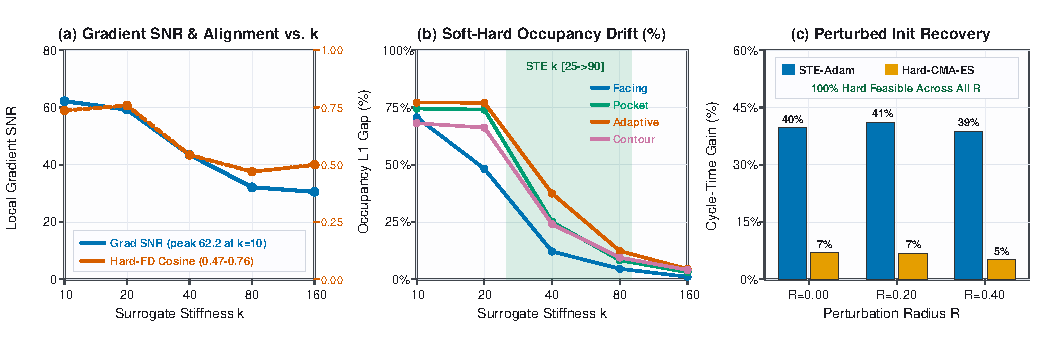
\includegraphics[width=\columnwidth]{figures/fig2_exp1_conditioning.pdf}
  \vspace{-1.6em}
  \caption{\textbf{Exp1: Surrogate gradient conditioning and perturbed recovery.} (a) Analytical gradient SNR ($62.2 \to 30.5$, blue) and hard finite-difference cosine ($0.76 \to 0.47$, orange right axis) across $k$. (b) Soft-to-hard occupancy $L_1$ bias collapses from $72.6\%$ ($k=10$) to $8.7\%$ ($k=80$) and $3.2\%$ ($k=160$) across our STE continuation window. (c) From perturbed initializations $R \in \{0.00, 0.20, 0.40\}$, \texttt{STE-Continuation-Adam} achieves $100\%$ feasibility and $38.7\%$--$41.1\%$ speedups vs.\ $5.1\%$--$6.9\%$ for \texttt{Hard-CMA-ES}.}
  \label{fig:exp1}
  \vspace{-0.8em}
\end{figure}

In Fig.~\ref{fig:exp1}(c), we perturb initial parameters uniformly within $\|\boldsymbol{\theta}_0\|_\infty \le R$ for $R \in \{0.00, 0.20, 0.40\}$ ($48$ simulator calls). \texttt{STE-Continuation-Adam} maintains $100\%$ hard feasibility across all $R$ and achieves $\mathbf{39.7\%}$, $\mathbf{41.1\%}$, and $\mathbf{38.7\%}$ cycle-time reductions—$5.8\times$ to $7.6\times$ the gain of zero-order \texttt{Hard-CMA-ES} ($6.9\%$, $6.7\%$, $5.1\%$).

\subsection{Exp2: Single-Task Trajectory and RL Benchmark}
Table~\ref{tab:exp2_main} and Fig.~\ref{fig:exp2_conv} report our main 16-task $\times$ 8-method benchmark under strict $B = 64$ simulator-call parity across 3 seeds ($100\%$ hard feasibility across all methods). Both smooth-to-hard continuation schedules substantially outperform fixed-stiffness and zero-order baselines, cutting mean cycle time from $122.20\text{ s}$ to $\mathbf{73.91\text{ s}}$ (\texttt{STE-Continuation-Adam}, $\mathbf{-42.0 \pm 13.5\%}$) and $\mathbf{73.74\text{ s}}$ (\texttt{Annealed-Adam}, $\mathbf{-43.0 \pm 15.7\%}$)—more than $10$ percentage points ahead of fixed-$k$ \texttt{Naive-Smooth-Adam} ($-31.9\%$, $83.44\text{ s}$) and nearly $4\times$ the speedup of evolutionary search (\texttt{Hard-CMA-ES} $-11.3\%$, \texttt{Hard-CEM} $-9.3\%$), which stall on $156$--$370$ segment Contour and Adaptive programs. Comparing our two continuation schedules under identical simulator calls exposes a clear compute-allocation trade-off: 1:1 per-step STE (\texttt{STE-Continuation-Adam}, $32$ gradient updates) achieves the highest speedups on engagement-varying \textbf{Facing} ($\mathbf{-59.7 \pm 1.2\%}$) and long-horizon trochoidal \textbf{Adaptive} clearing ($\mathbf{-37.3 \pm 7.2\%}$ vs.\ $-33.0\%$ for \texttt{Annealed-Adam}) while halving seed variance on walled \textbf{Pocket} roughing ($\pm 9.7\%$ vs.\ $\pm 19.2\%$), whereas 4:1 periodic hard checkpointing (\texttt{Annealed-Adam}, $51$ gradient updates) converts extra gradient steps into a lead on exterior \textbf{Contour} profiling ($\mathbf{-52.4 \pm 3.4\%}$).

\begin{table*}[t]
  \centering
  \caption{\textbf{Exp2 Main Benchmark across 16 Milling Tasks (4 Families $\times$ 4 Geometries $\times$ 3 Seeds, Strict Budget $B = 64$ Simulator Calls).} Cycle-time reductions ($-\Delta T_{\text{cycle}}$, $\%$) are mean $\pm$ std relative to \texttt{Nominal-CAM}; all methods achieve $100\%$ hard Boolean feasibility under blended acceleration kinematics.}
  \label{tab:exp2_main}
  \vspace{-0.4em}
  \resizebox{\textwidth}{!}{%
  \begin{tabular}{llccccccc}
    \toprule
    \textbf{Method} & \textbf{Optimization Class} & \textbf{Facing} ($\%$) & \textbf{Pocket} ($\%$) & \textbf{Adaptive} ($\%$) & \textbf{Contour} ($\%$) & \textbf{Overall $-\Delta T$} ($\%$) & \textbf{Mean $T$} (s) & \textbf{Peak MRR} ($\text{mm}^3$/s) \\
    \midrule
    \texttt{Nominal-CAM} & Clean-Room CAM Seed & $0.0 \pm 0.0$ & $0.0 \pm 0.0$ & $0.0 \pm 0.0$ & $0.0 \pm 0.0$ & $0.0 \pm 0.0$ & $122.20$ & $75.4$ \\
    \midrule
    \texttt{Hard-CEM}~\cite{rubinstein2004cem} & 0th-Order Elite Search & $15.6 \pm 2.6$ & $6.3 \pm 3.4$ & $6.1 \pm 1.2$ & $9.3 \pm 2.0$ & $9.3 \pm 4.5$ & $112.17$ & $88.8$ \\
    \texttt{Hard-CMA-ES}~\cite{hansen2001cmaes} & 0th-Order Covariance ES & $22.3 \pm 2.1$ & $6.3 \pm 3.5$ & $6.0 \pm 1.8$ & $10.6 \pm 3.4$ & $11.3 \pm 7.2$ & $110.62$ & $95.9$ \\
    \texttt{Hard-PPO}~\cite{schulman2017proximal} & 0th-Order Clipped RL & $21.0 \pm 3.4$ & $20.5 \pm 5.6$ & $10.1 \pm 4.4$ & $22.2 \pm 4.5$ & $18.5 \pm 6.6$ & $102.26$ & $93.9$ \\
    \midrule
    \texttt{Naive-Smooth-Adam} & 1st-Order Fixed $k=25$ & $33.6 \pm 8.1$ & $24.2 \pm 14.0$ & $33.3 \pm 4.4$ & $36.4 \pm 5.2$ & $31.9 \pm 9.9$ & $83.44$ & $105.9$ \\
    \texttt{DiffPolicy-SHAC}~\cite{xu2022accelerated} & 1st-Order Analytic RL & $53.6 \pm 2.8$ & $\mathbf{32.1 \pm 12.4}$ & $24.6 \pm 4.2$ & $37.7 \pm 2.6$ & $37.0 \pm 12.7$ & $81.67$ & $107.4$ \\
    \texttt{Annealed-Adam} & 1st-Order 4:1 $k$-Sched & $57.4 \pm 3.1$ & $29.2 \pm 19.2$ & $33.0 \pm 3.5$ & $\mathbf{52.4 \pm 3.4}$ & $\mathbf{43.0 \pm 15.7}$ & $\mathbf{73.74}$ & $109.7$ \\
    \texttt{STE-Continuation-Adam} & \textbf{1st-Order 1:1 STE (Ours)} & $\mathbf{59.7 \pm 1.2}$ & $26.9 \pm 9.7$ & $\mathbf{37.3 \pm 7.2}$ & $44.1 \pm 3.7$ & $\mathbf{42.0 \pm 13.5}$ & $73.91$ & $113.3$ \\
    \bottomrule
  \end{tabular}%
  }
  \vspace{-0.6em}
\end{table*}

\begin{figure*}[t]
  \centering
  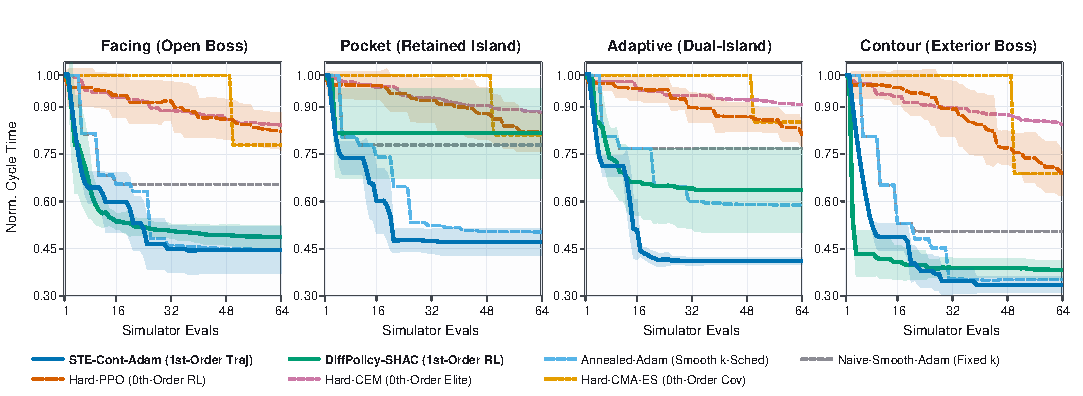
\includegraphics[width=\textwidth]{figures/fig3_exp2_convergence.pdf}
  \vspace{-1.6em}
  \caption{\textbf{Exp2 sample-efficiency convergence across clean-room CAM families ($B = 64$ simulator calls, mean $\pm$ 1 SD shaded).} First-order methods (\texttt{STE-Continuation-Adam}, \texttt{Annealed-Adam}, \texttt{DiffPolicy-SHAC}) achieve steep cycle-time reductions within the first $16$--$24$ calls by exploiting exact per-segment $\partial T_{\text{cycle}} / \partial f_t$ and $\partial \Delta V_t / \partial \mathbf{p}_t$ sensitivities, whereas zero-order RL (\texttt{Hard-PPO}) and evolutionary search (\texttt{Hard-CMA-ES}, \texttt{Hard-CEM}) progress slowly over $100$--$370$ segment horizons.}
  \label{fig:exp2_conv}
  \vspace{-0.8em}
\end{figure*}

Comparing our controlled RL arms directly answers the first- vs.\ zero-order policy learning question: under identical $64$--$64$ MLP architectures and a 64-call simulator budget, first-order \texttt{DiffPolicy-SHAC} achieves $\mathbf{-37.0 \pm 12.7\%}$ mean cycle-time reduction ($81.67\text{ s}$), \textbf{doubling ($2.0\times$)} the speedup of zero-order \texttt{Hard-PPO} ($\mathbf{-18.5 \pm 6.6\%}$, $102.26\text{ s}$) and more than tripling \texttt{Hard-CMA-ES} ($-11.3\%$). Because \texttt{Hard-PPO} must estimate credit assignment across up to $370$ sequential segments from Gaussian action noise, 64 rollouts provide only 8 policy updates. By contrast, \texttt{DiffPolicy-SHAC} backpropagates exact per-segment analytical sensitivities on every step—and notably achieves the \textbf{highest \texttt{Pocket} speedup of any method} ($\mathbf{-32.1 \pm 12.4\%}$ vs.\ $-26.9\%$ for spline-based STE) because its per-segment \texttt{DirectSegmentActionMap} accelerates individual corner-cleanup moves without B-spline basis smoothing across $92$--$169$ pocket segments.

\subsection{Exp3: Multi-Task Policy Transfer and Physical Ablations}
In \textbf{Exp3} (Table~\ref{tab:exp3_abl} top, Fig.~\ref{fig:exp3_abl}a), we train multi-task \texttt{DiffPolicy-SHAC} and \texttt{Hard-PPO} policies across the 8 \texttt{dev} tasks and evaluate generalization on the 8 unseen \texttt{test} tasks:
\begin{itemize}
  \item \textbf{Zero-Shot vs.\ Overload Trade-Off:} Across heterogeneous toolpath topologies ($37$-segment raster facing to $370$-segment trochoidal loops), zero-shot \texttt{DiffPolicy-SHAC} transfers strongly within low-horizon Facing ($\mathbf{+35.4\%}$ in $<\!1.5\text{ ms}$) while remaining conservative near nominal feeds on unseen multi-ring/trochoidal geometries ($8.3\%$ overall, $16.9\%$ MRR overload). Conversely, \texttt{Hard-PPO-ZeroShot} applies an aggressive uniform feed boost ($26.1\%$ speedup) that violates soft chip-load ratings with a $\mathbf{+24.5\%}$ Peak MRR overload ($133.2\text{ mm}^3/\text{s}$).
  \item \textbf{16-Call Few-Shot Adaptation:} Given just 16 test-time simulator calls, analytical gradients boost \texttt{DiffPolicy-SHAC-FewShot16} by $+19.4$ points to $\mathbf{27.7 \pm 15.8\%}$ while cutting MRR overload nearly $4\times$ ($16.9\% \to \mathbf{4.4\%}$), surpassing \texttt{Hard-PPO-FewShot16} ($23.4\%$, which degrades from zero-shot under noisy 4-batch exploration), while from-scratch \texttt{Scratch-STE-Adam-16} reaches $\mathbf{40.1 \pm 7.4\%}$ ($4.0\%$ overload).
\end{itemize}

\begin{table}[t]
  \centering
  \caption{\textbf{Top:} Exp3 Multi-Task Policy Transfer ($8$ Dev $\to$ $8$ Unseen Test Tasks, 3 Seeds). \textbf{Bottom:} Exp2 5-Arm Physical \& Kinematic Ablations ($8$ Test Tasks, $B = 64$). All arms achieve $100\%$ geometric feasibility; removing the MRR barrier triggers $+136.7\%$ cutter overload.}
  \label{tab:exp3_abl}
  \vspace{-0.4em}
  \resizebox{\columnwidth}{!}{%
  \begin{tabular}{lcccc}
    \toprule
    \textbf{Regime / Ablation Arm} & \textbf{Calls} & \textbf{$-\Delta T_{\text{cycle}}$} ($\%$) & \textbf{Peak MRR} & \textbf{Overload} \\
    \midrule
    \multicolumn{5}{l}{\emph{Exp3: Unseen Test Policy Generalization}} \\
    \texttt{Hard-PPO-ZeroShot} & $1$ & $26.1 \pm 9.5$ & $133.2$ & $24.5\%$ \\
    \texttt{DiffPolicy-SHAC-ZeroShot} & $1$ & $8.3 \pm 17.9$ & $124.9$ & $16.9\%$ \\
    \texttt{Hard-PPO-FewShot16} & $16$ & $23.4 \pm 9.5$ & $104.9$ & $2.7\%$ \\
    \texttt{DiffPolicy-SHAC-FewShot16} & $16$ & $\mathbf{27.7 \pm 15.8}$ & $111.4$ & $4.4\%$ \\
    \texttt{Scratch-STE-Adam-16} & $16$ & $\mathbf{40.1 \pm 7.4}$ & $114.4$ & $4.0\%$ \\
    \midrule
    \multicolumn{5}{l}{\emph{Exp2-Abl: Physical \& Kinematic Ablations ($B = 64$)}} \\
    \texttt{Path-Only-Frozen-Feed} & $64$ & $0.2 \pm 0.4$ & $82.1$ & $0.0\%$ \\
    \texttt{Full-Joint-Blended-STE} & $64$ & $37.0 \pm 17.9$ & $114.9$ & $\mathbf{5.2\%}$ \\
    \texttt{Exact-Stop-Surrogate} & $64$ & $39.2 \pm 18.2$ & $109.6$ & $2.3\%$ \\
    \texttt{Feed-Only-Frozen-Path} & $64$ & $\mathbf{39.5 \pm 13.7}$ & $118.7$ & $7.3\%$ \\
    \texttt{No-MRR-Barrier} ($w_{\text{MRR}}\!=\!0$) & $64$ & $66.2 \pm 3.5$ & $\mathbf{262.6}$ & $\mathbf{136.7\%}$ \\
    \bottomrule
  \end{tabular}%
  }
  \vspace{-0.8em}
\end{table}

\begin{figure}[t]
  \centering
  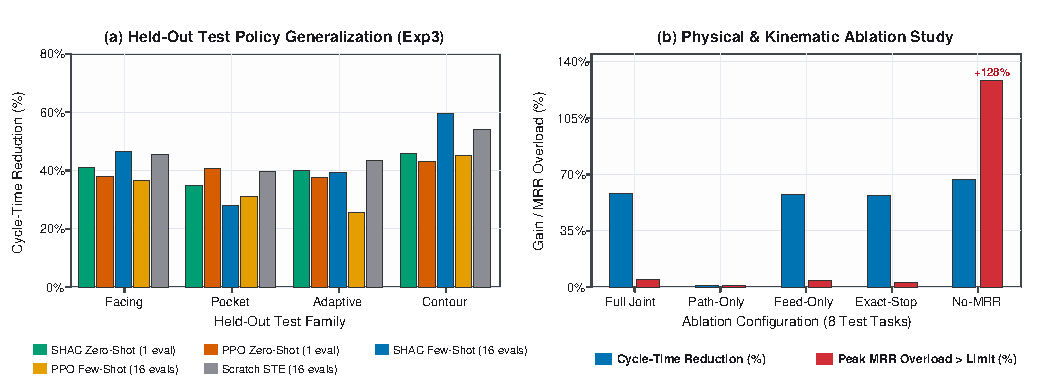
\includegraphics[width=\columnwidth]{figures/fig4_exp3_transfer_ablations.pdf}
  \vspace{-1.6em}
  \caption{\textbf{Exp3 policy generalization and physical ablations.} (a) Held-out test cycle-time reductions across families for zero-shot ($1$ call) and few-shot ($16$ calls) transfer. (b) Ablating feed optimization (\texttt{Path-Only}) collapses gains to $0.2\%$, whereas ablating the volumetric MRR barrier (\texttt{No-MRR}) triggers $+136.7\%$ peak cutter overload.}
  \label{fig:exp3_abl}
  \vspace{-0.8em}
\end{figure}

Our 5-arm ablation on the 8 held-out test tasks (Table~\ref{tab:exp3_abl} bottom, Fig.~\ref{fig:exp3_abl}b) confirms three core physical hypotheses: (1) \texttt{Path-Only-Frozen-Feed} yields only $\mathbf{0.2 \pm 0.4\%}$ speedup because clean-room stepovers and blueprint walls lock pass topology under constant feedrates; (2) under $32$ STE updates ($B=64$), joint XY-and-feed co-optimization (\texttt{Full-Joint-Blended-STE}, $37.0\%$) matches \texttt{Feed-Only-Frozen-Path} ($39.5\%$) and \texttt{Exact-Stop-Surrogate} ($39.2\%$) within variance while reducing Peak MRR overload by $\mathbf{29\%}$ relative to frozen-path feed scheduling ($\mathbf{5.2\%}$ vs.\ $7.3\%$, $114.9$ vs.\ $118.7\text{ mm}^3/\text{s}$) by laterally easing roughing engagement; and (3) setting $w_{\text{MRR}} = 0$ (\texttt{No-MRR-Barrier}) inflates apparent gain to $66.2\%$ by commanding $v_{\max}$ through full-width slotting cuts, driving mean peak MRR to $\mathbf{262.6\text{ mm}^3/\text{s}}$ ($\mathbf{+136.7\%}$ overload).

\subsection{Exp4: Multi-Controller NC, CAMotics STL, and Simulator Audit}
To verify that optimization on a $0.50\text{ mm}$ grid introduces zero discretization or post-processing regressions, Table~\ref{tab:exp4} audits all 8 held-out test parts compiled into Haas Mini Mill Next-Gen Control programs (\texttt{O01001}--\texttt{O01008}, \texttt{G54}, \texttt{G187 P2 E0.05}) and across all 6 industrial CNC dialects ($48$ programs total). Mean test cycle time drops from $\mathbf{128.80\text{ s}}$ to $\mathbf{82.13\text{ s}}$ ($\mathbf{-36.2\%}$ total machining time, $\mathbf{-39.5\%}$ unweighted mean per part, up to $\mathbf{-60.9\%}$ on \texttt{face-test-01}). Every single program across all $48/48$ controller outputs passes our $0.25\text{ mm}$-voxel, $0.125\text{ mm}$-step \texttt{posted\_evaluator} geometric and holder/rapid safety screen with \textbf{exactly $\mathbf{0.00\text{ mm}^3}$ target gouge and $\mathbf{0.00\text{ mm}^3}$ uncut residual}. Independently, containerized \texttt{CAMotics v1.2.0} reconstructs $\mathbf{8/8}$ closed, manifold, watertight STL solids ($72{,}576$--$129{,}296$ facets) whose enclosed volumes and facet counts match \texttt{Nominal-CAM} identically ($\Delta V = \mathbf{0.000\%}$ on every part), all inspectable interactively alongside 3D toolpaths in our \texttt{.rustcnc}, \texttt{.camotics}, and WebGL simulator bundles.

\begin{table*}[t]
  \centering
  \caption{\textbf{Exp4 Independent High-Resolution Verification, 6-Controller Audit, and Haas Mini Mill NGC Shop Packet Summary Across All 8 Held-Out Test Parts.} Audited on posted G-code across 6 dialects (\texttt{RS274}, Haas NGC \texttt{G187 P2 E0.05}, \texttt{FANUC}, \texttt{Robodrill}, \texttt{Makino}, \texttt{Mazak}; $48/48$ pass) via a $0.125\text{ mm}$-step \texttt{posted\_evaluator} ($0.25\text{ mm}$ voxels) and containerized \texttt{CAMotics v1.2.0} ($0.25\text{ mm}$ octree STL reconstruction).}
  \label{tab:exp4}
  \vspace{-0.4em}
  \resizebox{\textwidth}{!}{%
  \begin{tabular}{lllccccccccc}
    \toprule
    \textbf{Haas Prog.} & \textbf{Case ID} & \textbf{CAM Family} & \textbf{Stock} (mm) & \textbf{$T_{\text{nom}}$} (s) & \textbf{$T_{\text{DiffCAM}}$} (s) & \textbf{$-\Delta T$} ($\%$) & \textbf{Gouge} ($\text{mm}^3$) & \textbf{Res.} ($\text{mm}^3$) & \textbf{6-Dialect} & \textbf{CAMotics STL} & \textbf{STL Vol.} ($\text{mm}^3$) \\
    \midrule
    \texttt{O01001} & \texttt{face-test-00} & Facing Boss & $34\!\times\!24\!\times\!8$ & $79.92$ & $32.85$ & $58.9\%$ & $0.00$ & $0.00$ & $6/6$ Pass & Watertight ($74.9\text{k}\triangle$) & $4245.9$ \\
    \texttt{O01002} & \texttt{face-test-01} & Facing Boss & $32\!\times\!24\!\times\!8$ & $77.68$ & $30.34$ & $60.9\%$ & $0.00$ & $0.00$ & $6/6$ Pass & Watertight ($72.6\text{k}\triangle$) & $4370.6$ \\
    \texttt{O01003} & \texttt{pocket-test-00} & Pocket Island & $32\!\times\!28\!\times\!8$ & $117.24$ & $96.26$ & $17.9\%$ & $0.00$ & $0.00$ & $6/6$ Pass & Watertight ($107.9\text{k}\triangle$) & $5034.5$ \\
    \texttt{O01004} & \texttt{pocket-test-01} & Pocket Island & $34\!\times\!26\!\times\!8$ & $89.94$ & $62.01$ & $31.0\%$ & $0.00$ & $0.00$ & $6/6$ Pass & Watertight ($102.1\text{k}\triangle$) & $5514.2$ \\
    \texttt{O01005} & \texttt{adapt-test-00} & Adaptive Trochoid & $38\!\times\!30\!\times\!8$ & $188.64$ & $123.36$ & $34.6\%$ & $0.00$ & $0.00$ & $6/6$ Pass & Watertight ($129.3\text{k}\triangle$) & $6675.4$ \\
    \texttt{O01006} & \texttt{adapt-test-01} & Adaptive Trochoid & $36\!\times\!32\!\times\!8$ & $280.60$ & $198.18$ & $29.4\%$ & $0.00$ & $0.00$ & $6/6$ Pass & Watertight ($127.1\text{k}\triangle$) & $7060.9$ \\
    \texttt{O01007} & \texttt{contour-test-00} & Contour Boss & $32\!\times\!26\!\times\!8$ & $107.81$ & $59.82$ & $44.5\%$ & $0.00$ & $0.00$ & $6/6$ Pass & Watertight ($76.1\text{k}\triangle$) & $4143.0$ \\
    \texttt{O01008} & \texttt{contour-test-01} & Contour Boss & $32\!\times\!24\!\times\!8$ & $88.60$ & $54.19$ & $38.8\%$ & $0.00$ & $0.00$ & $6/6$ Pass & Watertight ($73.2\text{k}\triangle$) & $4204.8$ \\
    \midrule
    \textbf{Mean / Pass} & \multicolumn{3}{l}{\textbf{8 Held-Out Test Parts ($36.2\%$ Agg.\ Time Saved)}} & $\mathbf{128.80}$ & $\mathbf{82.13}$ & $\mathbf{39.5\%}$ & $\mathbf{0.00}$ & $\mathbf{0.00}$ & $\mathbf{48/48}$ & $\mathbf{8/8}$ \textbf{Watertight} & $\Delta V = 0.000\%$ \\
    \bottomrule
  \end{tabular}%
  }
  \vspace{-0.8em}
\end{table*}

\section{Limitations and Conclusion}
\label{sec:conclusion}

\textbf{Limitations.}
First, our current parameterization locks axial coordinates $\bar{p}_i^z$ to canonical 2.5D cutting layers; extending wall-clearance mobility weights to simultaneous 3-axis ball-endmill sculptured surfacing and 5-axis tool-orientation smoothing is a natural next step. Second, while our volumetric Peak MRR barrier prevents steady-state chip-load and torque overload, it does not model frequency-domain regenerative chatter lobes~\cite{altintas2012manufacturing} or thin-wall deflection. Third, although \texttt{DiffPolicy-SHAC} achieves $2.0\times$ single-task sample efficiency over \texttt{Hard-PPO} and rapid 16-call adaptation across unseen geometries, zero-shot generalization across wildly varying horizon lengths ($37$--$370$ segments) motivates graph or transformer toolpath backbones, and topology-changing pass insertion still relies on upstream geometric CAM seeding. Finally, while our Haas Mini Mill NGC shop packets (\texttt{O01001}--\texttt{O01008}) are certified in \texttt{CAMotics v1.2.0} and high-resolution swept-SDF simulation, instrumented physical Al 6061-T6 cutting trials measuring spindle load and profilometry roughness constitute our immediate hardware milestone.

\textbf{Conclusion.}
We presented \textbf{DiffCAM}, an MIT-licensed dual-mode differentiable 3-axis milling simulator, clean-room CAM suite, and co-optimization framework that reconciles discontinuous Boolean CSG geometry with smooth analytical policy and trajectory gradients. By combining Straight-Through Estimator stiffness continuation, controller-matched corner-blending kinematics, volumetric Peak MRR barriers, and drift-free \texttt{JointPathFeedSpline} parameterizations, DiffCAM achieves $42\%$--$43\%$ mean cycle-time reductions at $100\%$ feasibility, demonstrates a $2.0\times$ sample-efficiency advantage for first-order differentiable RL over zero-order RL, and delivers certified watertight \texttt{CAMotics} STL solids, interactive 3D simulator workspaces, and shop-ready 6-controller G-code.

\bibliographystyle{plainnat}
{\small
\setlength{\bibsep}{2.5pt}
\bibliography{references}
}

\end{document}
